\documentclass[a4paper,12pt]{article}
\usepackage[super,square]{natbib}
% Package to change margin size
\usepackage{anysize}
\usepackage{amsmath}
\marginsize{2cm}{2cm}{1cm}{2cm}
\usepackage{fancyhdr}
\usepackage{circuitikz}
\renewcommand{\headrulewidth}{0pt}
\usepackage{soul}
\usepackage[section]{placeins}
% Colors for the references links
\usepackage[dvipsnames]{xcolor}
% Package to link references
\usepackage{hyperref}
\usepackage{graphicx}
\usepackage{float}
\hypersetup{
 colorlinks=true,
  linkcolor=black,
  citecolor=CadetBlue,  
  filecolor=CadetBlue,      
  urlcolor=CadetBlue,
}
% Package for lorem ipsum
\usepackage{lipsum}
% Package for multicolumn
\usepackage{multicol}
% Package for removing paragraph identations
\usepackage{parskip}
\usepackage{booktabs}
\setlength\columnsep{18pt}
% Sets bastract
\renewenvironment{abstract}
{\par\noindent\textbf{\abstractname}\ \ignorespaces \\}
{\par\noindent\medskip}




\begin{document}
% Makes header
\pagestyle{fancy}
\thispagestyle{empty}
\fancyhead[R]{\textit{EE1200}}
\fancyhead[L]{}
% Makes footnotes with an asterisk
\renewcommand*{\thefootnote}{\fnsymbol{footnote}}
\begin{center}
    \Large{\textbf{Experiment 07}}
    \vspace{0.4cm}
    \normalsize
    \\ Aditya Tripathy - ee24btech11001, Durgi Swaraj Sharma - ee24btech11018\\
    \medskip
    \normalsize
\end{center}
{\color{gray}\hrule}
\vspace{0.4cm}
\begin{abstract}
    In Experiment-07, we used T Flip-Flops(FFs) to make a Mod-7 Asynchronous Counter, with the help of a NAND gate. 
\end{abstract}
{\color{gray}\hrule}
\medskip
\section{Objective}
To design a Mod-7 Asynchronous Counter using T Flip-Flops and demonstrate its performance using a Cathode Ray Oscilloscope with a clock from an Arduino.
\section{Apparatus}
\begin{itemize}
    \item 3x T Flip-Flops [we had no access to T Flip-Flops, so we used JK Flip-Flops HD74LS76AP with appropriate changes to make them function like a T FF.]
    \item 3x LEDs
    \item 3-input NAND gate [we used DM74LS10]
    \item Oscilloscope
    \item Arduino
    \item DC power supply
    \item Connecting wires and probes
\end{itemize}
\section{Theory and Circuit}

Counters are sequential circuits that store the number of times an event has occured. They can have a sequence, like counting in binary numbers. Up counters count in incrementing fashion, while down counters count in decrementing fashion. They can be made using Flip-Flops and a clock signal.  

In Asynchronous Counters, only the first FF gets the clock signal, and the following FFs are driven by the outputs of the previous FFs. The FFs are cascaded, and the changes propagate in a Ripple fashion.

Using T FFs, asynchronous counters can be contructed by using one FFs output $Q$ as the clock signal for the next, while maintaining $T$ at HIGH. If the FFs are positive edge triggered, this design will be a down counter, and if the FFs are negative edge triggered, this desgin will be an up counter. Up and down counters can be changed to their opposite types by inverting the output signal of the FFs before it is used to drive the next FF.

We want to design a Mod-7 counter wil the T FFs. That means we want our counter to count between the numbers possible from a mod-7 operation: 0,1,2,3,4,5,6. The minimum number of FFs needed for this would be 3, with which we will be able to represent numbers from 0-7. But we want the counter to set to 0 after 6, instead of the default behaviour of counting to 7 and then setting to 0. For this functioning we shall employ the use of the $\overline{clr}$ pins of the FF, when when set to a LOW will set the FF output to 0. Note that $\overline{pre}$ should remain at a HIGH throught our circuit and operation, and $\overline{clr}$ should only go LOW when the counter reaches 7, or 111 in binary. This condition is checked using a NAND gate to perform the operation $(Q_0Q_1Q_2)^{\prime}$ and using this as the $\overline{clr}$ signal. 

Based on these ideas, the circuit can be realized with positive edge triggered FFs as follows.
\begin{figure}[H]
    \centering
    \resizebox{1 \textwidth}{!}{
	\begin{circuitikz}
	    \draw (3.75,13.25) rectangle (6.25,9.5);
	    \draw (7.5,13.25) rectangle (10,9.5);
	    \draw (11.25,13.25) rectangle (13.75,9.5);
	    \draw (7,12.75) to[short] (7.5,12.75);
	    \draw (3.25,12.75) to[short] (3.75,12.75);
	    \draw (10.75,12.75) to[short] (11.25,12.75);
	    \draw (3.75,10.75) to[short] (4.25,10.75);
	    \draw (4.25,10.75) to[short] (3.75,10.25);
	    \draw (7.5,10.75) to[short] (8,10.75);
	    \draw (8,10.75) to[short] (7.5,10.25);
	    \draw (11.25,10.75) to[short] (11.75,10.75);
	    \draw (11.75,10.75) to[short] (11.25,10.25);
	    \draw (6.25,12) to[short] (6.75,12);
	    \draw (6.75,12) to[short] (6.75,10.75);
	    \draw (10,12) to[short] (10.5,12);
	    \draw (10.5,12) to[short] (10.5,10.75);
	    \draw (13.75,12) to[short] (14.25,12);
	    \draw (6.5,12) to[short] (6.5,9);
	    \draw (10.25,12) to[short] (10.25,9);
	    \draw (14,12) to[short] (14,9);
	    \draw (6.5,9) to[short] (10,9);
	    \draw (14,9) to[short] (10.5,9);
	    \draw (10,9) to[short] (10,8.25);
	    \draw (10.5,9) to[short] (10.5,8.25);
	    \draw (10.25,9) to[short] (10.25,8.25);
	    \draw (10,8.25) to[short] (10,6.75);
	    \draw (10.75,7.25) to[short] (11.5,7.25);
	    \draw (10.75,6.75) to[short] (11.5,6.75);
	    \draw (11.5,7.25) node[ieeestd nand port, anchor=in 1, scale=0.89](port){} (port.out) to[short] (14,7);
	    \draw (10.75,6.75) to[short] (10,6.75);
	    \draw (10.25,8.25) to[short] (10.25,7);
	    \draw (10.25,7) to[short] (11.75,7);
	    \draw (10.5,8.25) to[short] (10.5,7.25);
	    \draw (10.5,7.25) to[short] (11,7.25);
	    \draw (14,7) to[short] (16.25,7);
	    \draw (16.25,7) to[short] (16.25,14.5);
	    \draw (16.25,14.5) to[short] (5.75,14.5);
	    \draw (6.75,10.75) to[short, -o] (7.5,10.75) ;
	    \draw (10.5,10.75) to[short, -o] (11.25,10.75) ;
	    \draw (3,10.75) to[short, -o] (3.75,10.75) ;
	    \node [font=\normalsize] at (7,12) {$Q_0$};
	    \node [font=\normalsize] at (10.75,12) {$Q_1$};
	    \node [font=\normalsize] at (14.5,12) {$Q_2$};
	    \node [font=\small] at (3.25,13) {$T=1$};
	    \node [font=\small] at (7,13) {$T=1$};
	    \node [font=\small] at (10.75,13) {$T=1$};
	    \draw (5,14) to[short, -o] (5,13.25) ;
	    \draw (8.75,14) to[short, -o] (8.75,13.25) ;
	    \draw (12.5,14) to[short, -o] (12.5,13.25) ;
	    \draw (5.75,14.5) to[short, -o] (5.75,13.25) ;
	    \draw (9.5,14.5) to[short, -o] (9.5,13.25) ;
	    \draw (13.25,14.5) to[short, -o] (13.25,13.25) ;
	    \node [font=\small] at (4.75,13) {$\overline{pre}$};
	    \node [font=\small] at (8.5,13) {$\overline{pre}$};
	    \node [font=\small] at (12.5,13) {$\overline{pre}$};
	    \draw (2.5,12.75) to[short] (3.25,12.75);
	    \node [font=\small] at (5.75,13) {$\overline{clr}$};
	    \node [font=\small] at (9.5,13) {$\overline{clr}$};
	    \node [font=\small] at (13.25,13) {$\overline{clr}$};
	\end{circuitikz}}
	\caption{Mod-7 counter}
\end{figure}


\section{Procedure}
\subsection{The Circuit}
Before we even begin building the circuit, we should be aware of the specifications of the ICs we're working with. For that we should refer to the datasheets. 

In our case, the HD74LS76AP is a negative edge triggered JK Flip-FLop, and that means we don't need to use a signal inverter before we use the outputs as the next FF's clock signals for an up counter implementation. It otherwise functions like any JK Flip-Flop, and to use it as a T FF we just need to use both the J and K pins as T (J=T, K=T), and set them to HIGH to use as a counter. 
\begin{itemize}
    \item Connect the J K pins of the three FFs to HIGH(5V). 
\end{itemize}	
The DM74LS10 has multiple simple 3-input NAND gates of which we need to use only one for the $clr$ condition.
\begin{itemize}
    \item Connect the outputs of the three FFs $Q_0$, $Q_1$, $Q_2$ to three inputs of the NAND gate. (Make sure you're using the same NAND gate on the IC)
    \item Connect the output of the NAND gate to the $\overline{clr}$ pins of the three FFs.
    \item Set the $\overline{pre}$ pins of the FFs to HIGH.
    \item Connect GND to ground, and $V_{cc}$ to the appropriate power voltages for the ICs as given in the datasheets. 
\end{itemize}
We shall use an Arduino to generate the clock signal. Runnning the following code on an Arduino gives us a 1Hz square wave signal from pin D13.

\begin{verbatim}
#include <Arduino.h>

void squareWave()
{
  digitalWrite(13, 1);
  delay(500);
  digitalWrite(13, 0);
  delay(500);
}
void setup() {
    pinMode(13, OUTPUT);  
}

void loop() {
    squareWave();
}
\end{verbatim}
\begin{itemize}
    \item Connect the D13 pin of the Arduino to the clock(clk) pin of the first FF.
    \item Because our FFs are negative edge triggered, just connect the FF outputs to the clk pins of the next FFs directly.
\end{itemize}
\subsection{Visualizing the Operation}
We will use 3 LEDs to visualize the outputs of the FFs. The LEDs will light up when the output signal is high, helping us visualize the bits of the counter.
\begin{itemize}
    \item Connect the longer pins of the LEDs to the output pins of the Flip-Flops, and the other pin to ground
\end{itemize}
The FFs have enough internal resistance to not burn the LEDs.

To study the signals over time, we shall use a dual-channel oscilloscope.
\begin{itemize}
    \item Connect one of the probes to measure the arduino clock signal
    \item Connect the other probe to measure the output signal of the first FF.
    \item Observe the signals on the oscilloscope, and repeat for the other two output signals
\end{itemize}
\section{Observations}
\begin{figure}[H]
    \centering
    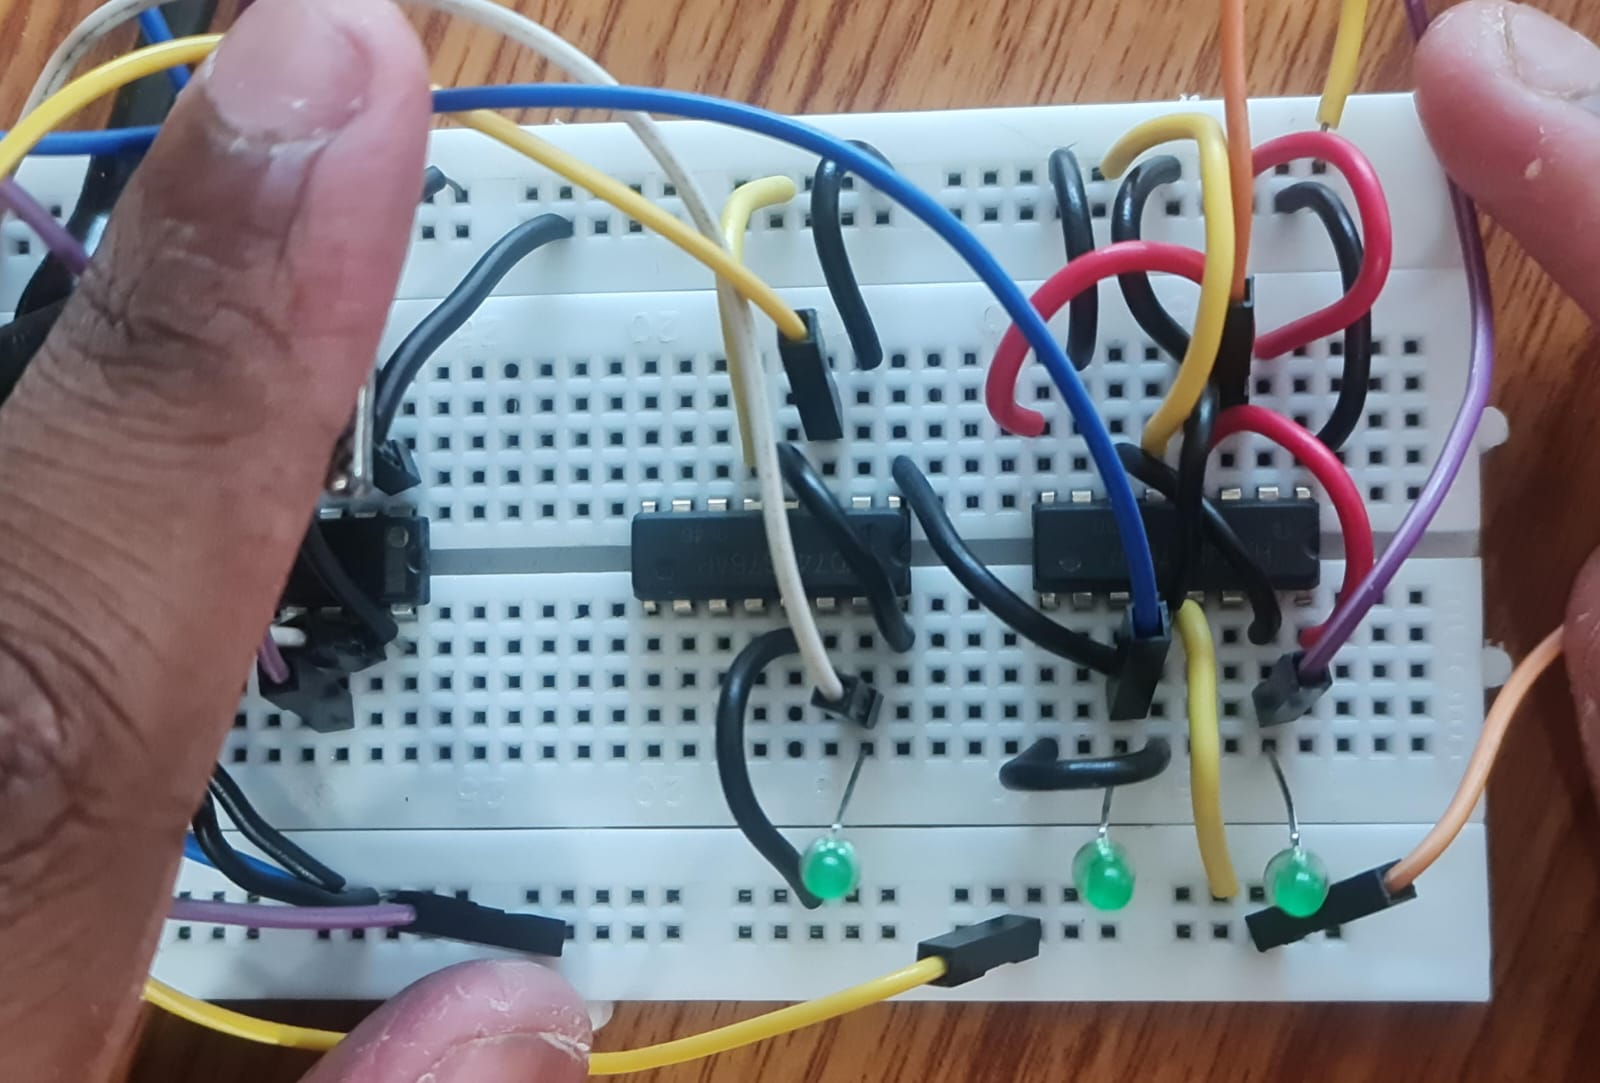
\includegraphics[width = 0.3\columnwidth]{figs/0.jpeg}
    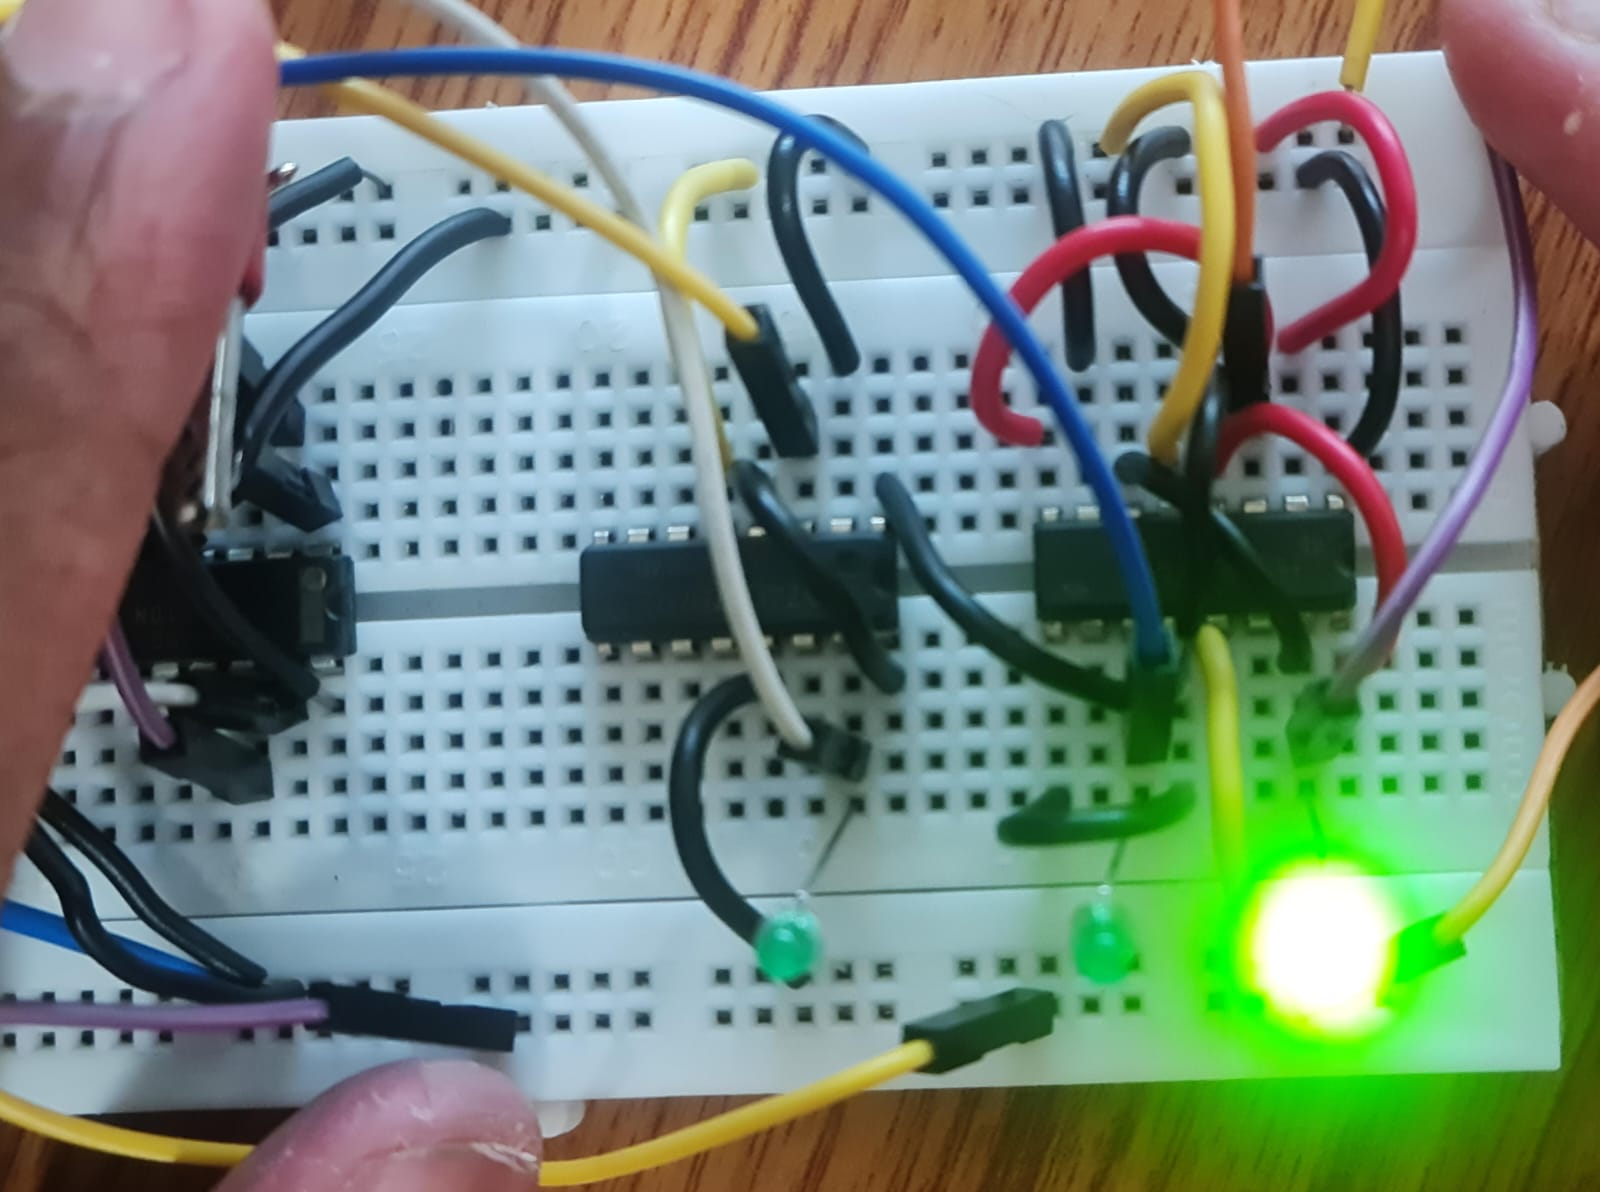
\includegraphics[width = 0.3\columnwidth]{figs/1.jpeg}
    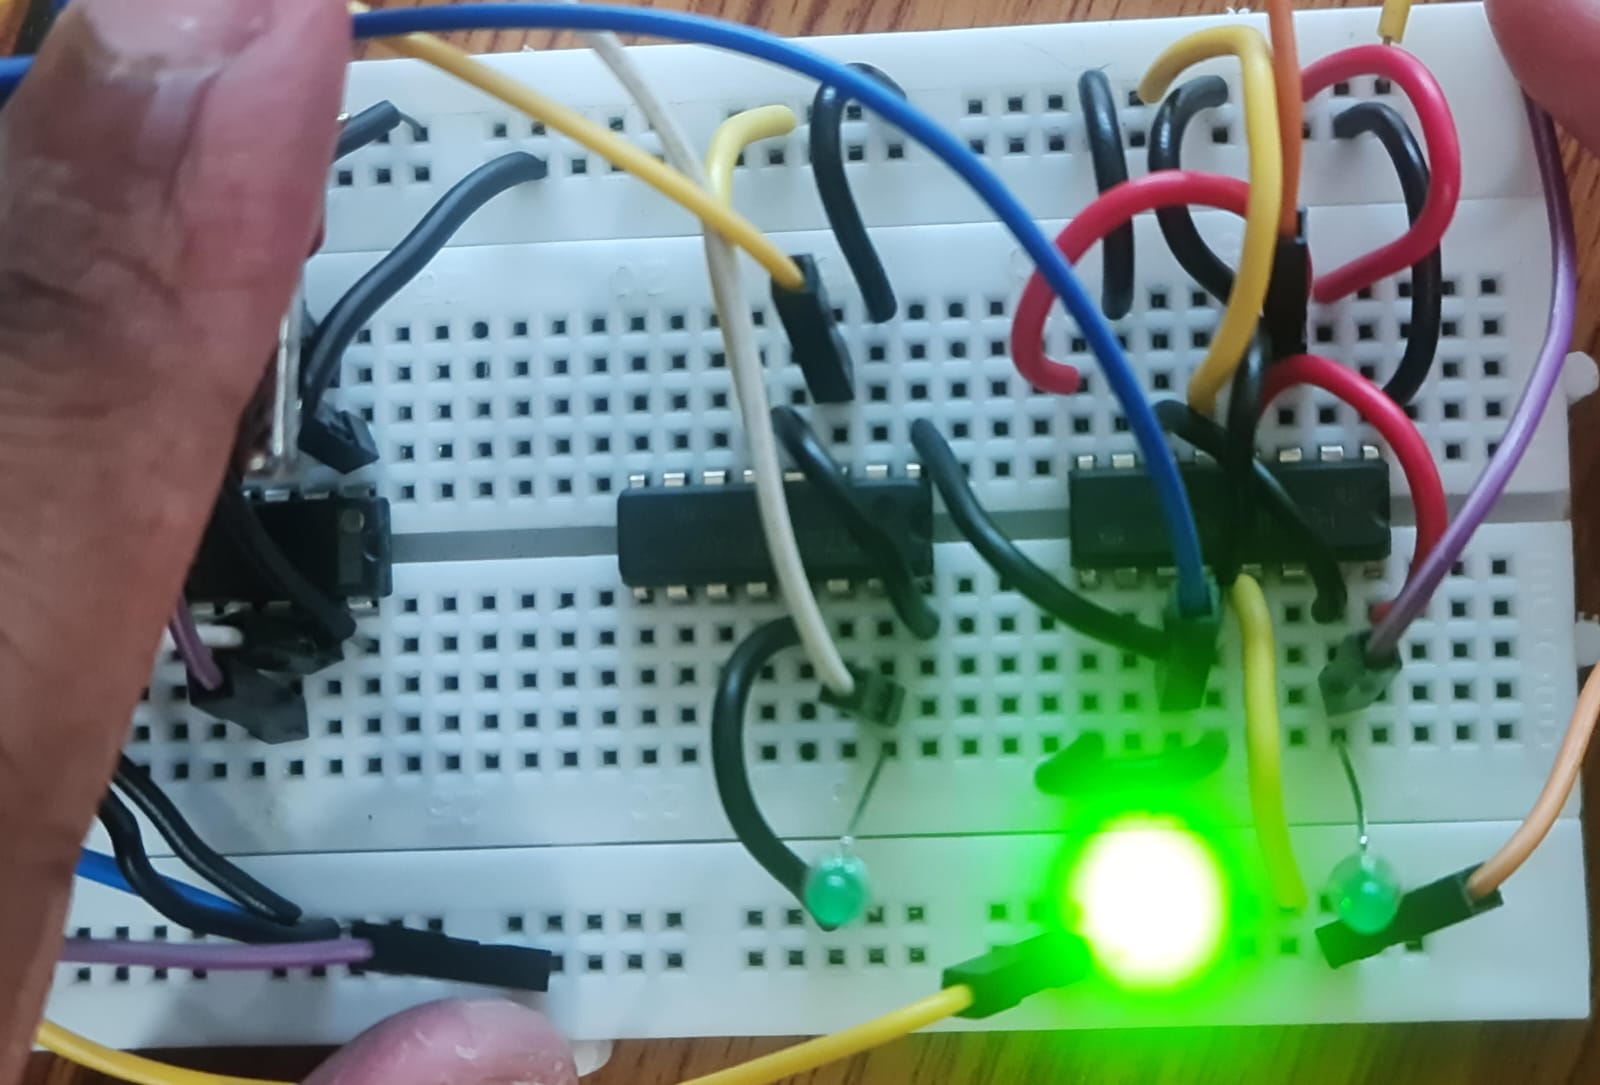
\includegraphics[width = 0.3\columnwidth]{figs/2.jpeg}
    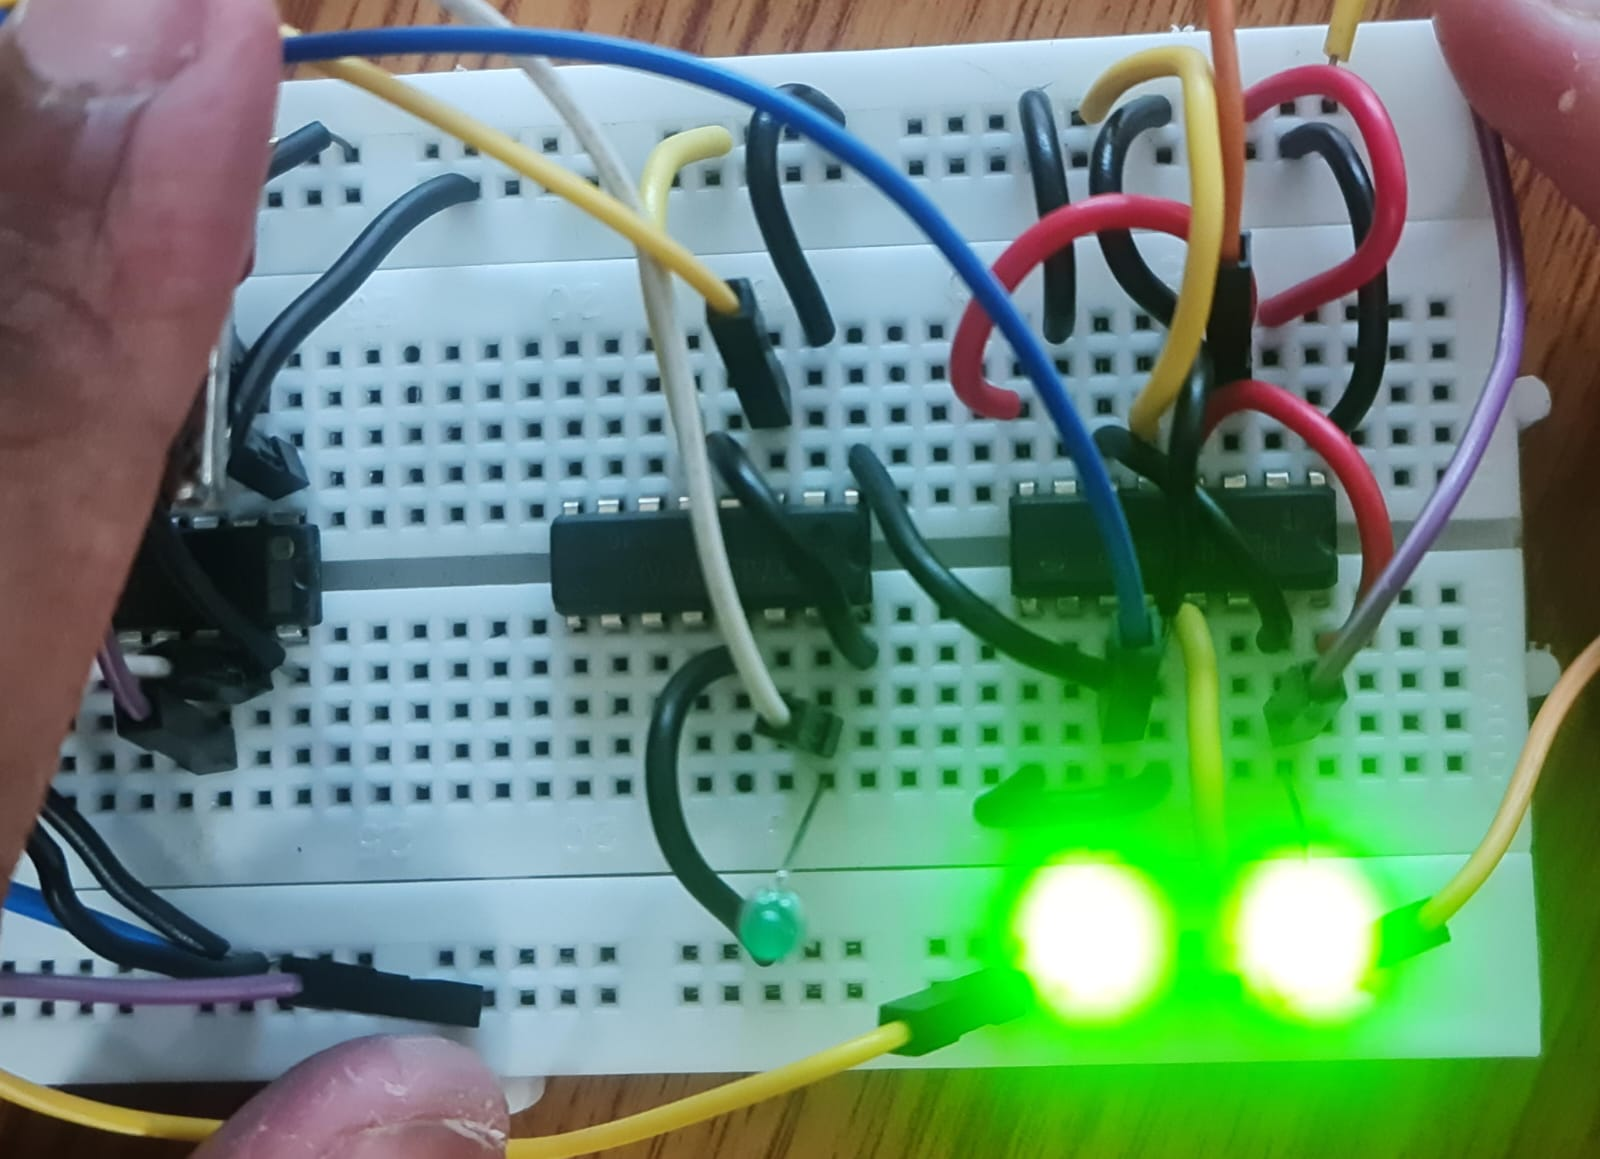
\includegraphics[width = 0.3\columnwidth]{figs/3.jpeg}
    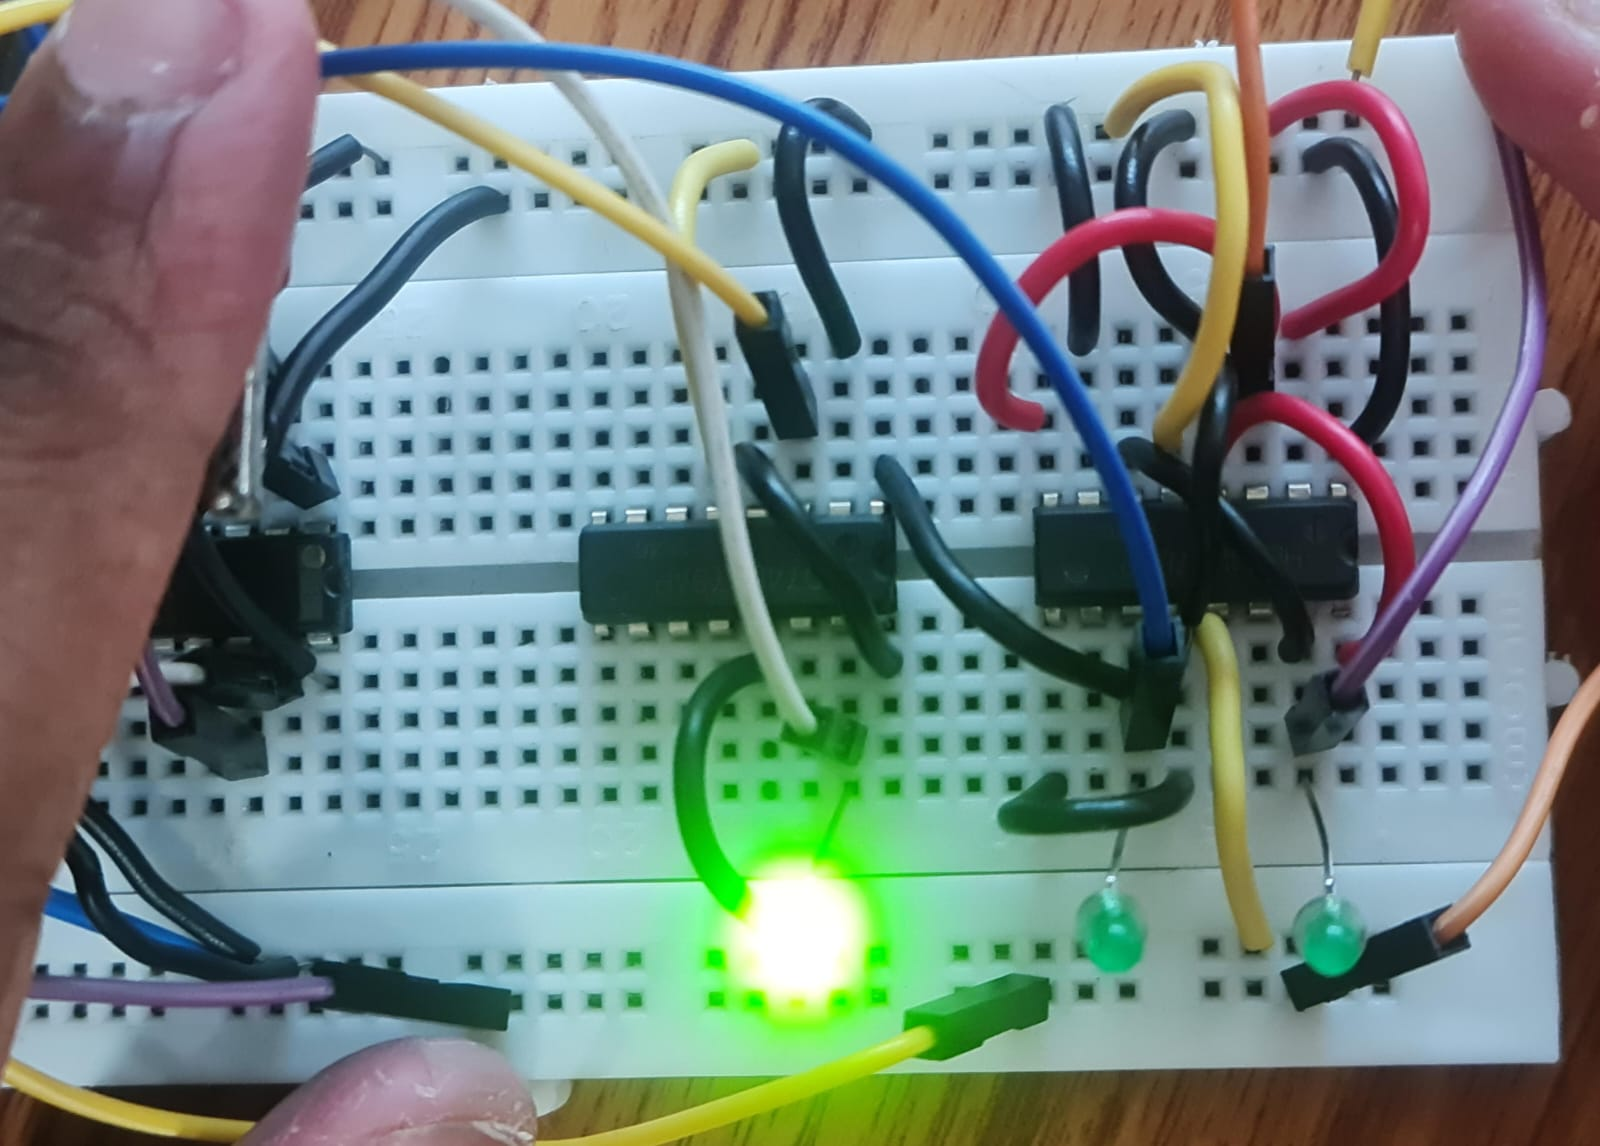
\includegraphics[width = 0.3\columnwidth]{figs/4.jpeg}
    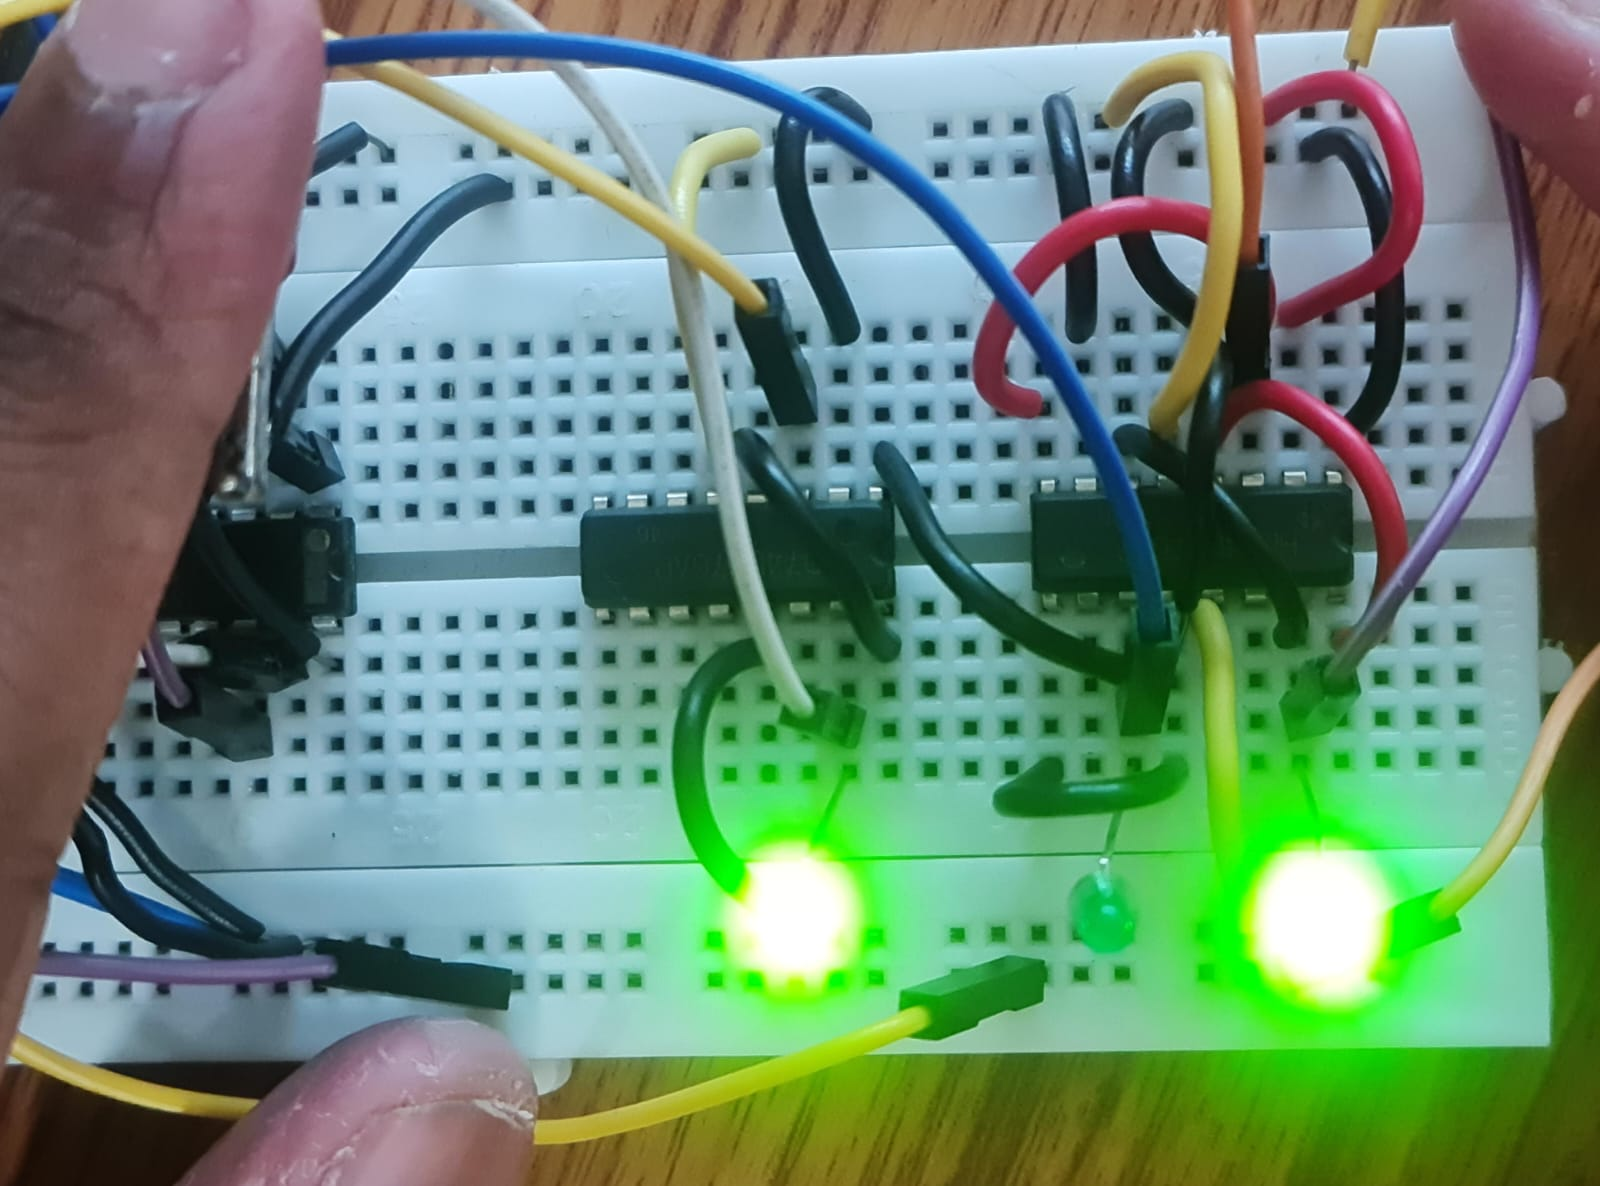
\includegraphics[width = 0.3\columnwidth]{figs/5.jpeg}
    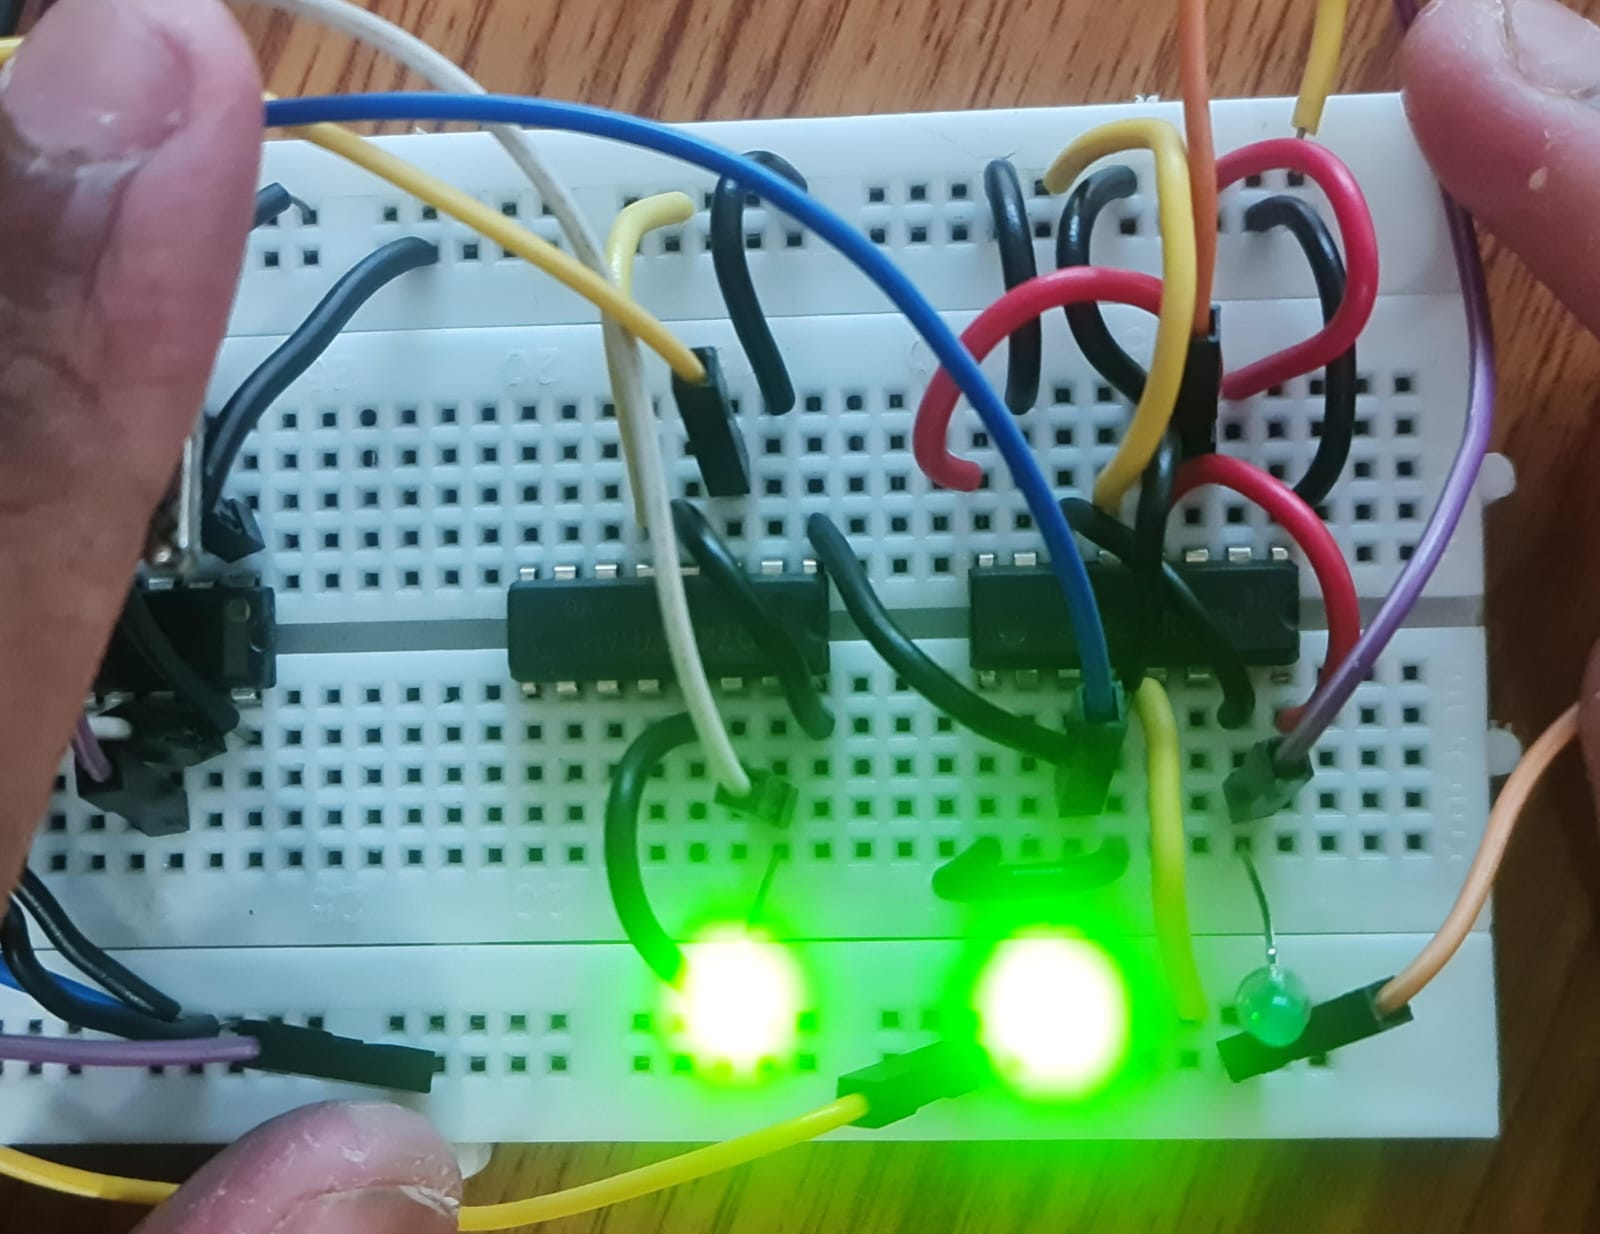
\includegraphics[width = 0.3\columnwidth]{figs/6.jpeg}
    \caption{Numbers 0-6 represented on the LEDs in binary, bit of least significance on the right.}
\end{figure}
\begin{figure}[H]
    \centering
    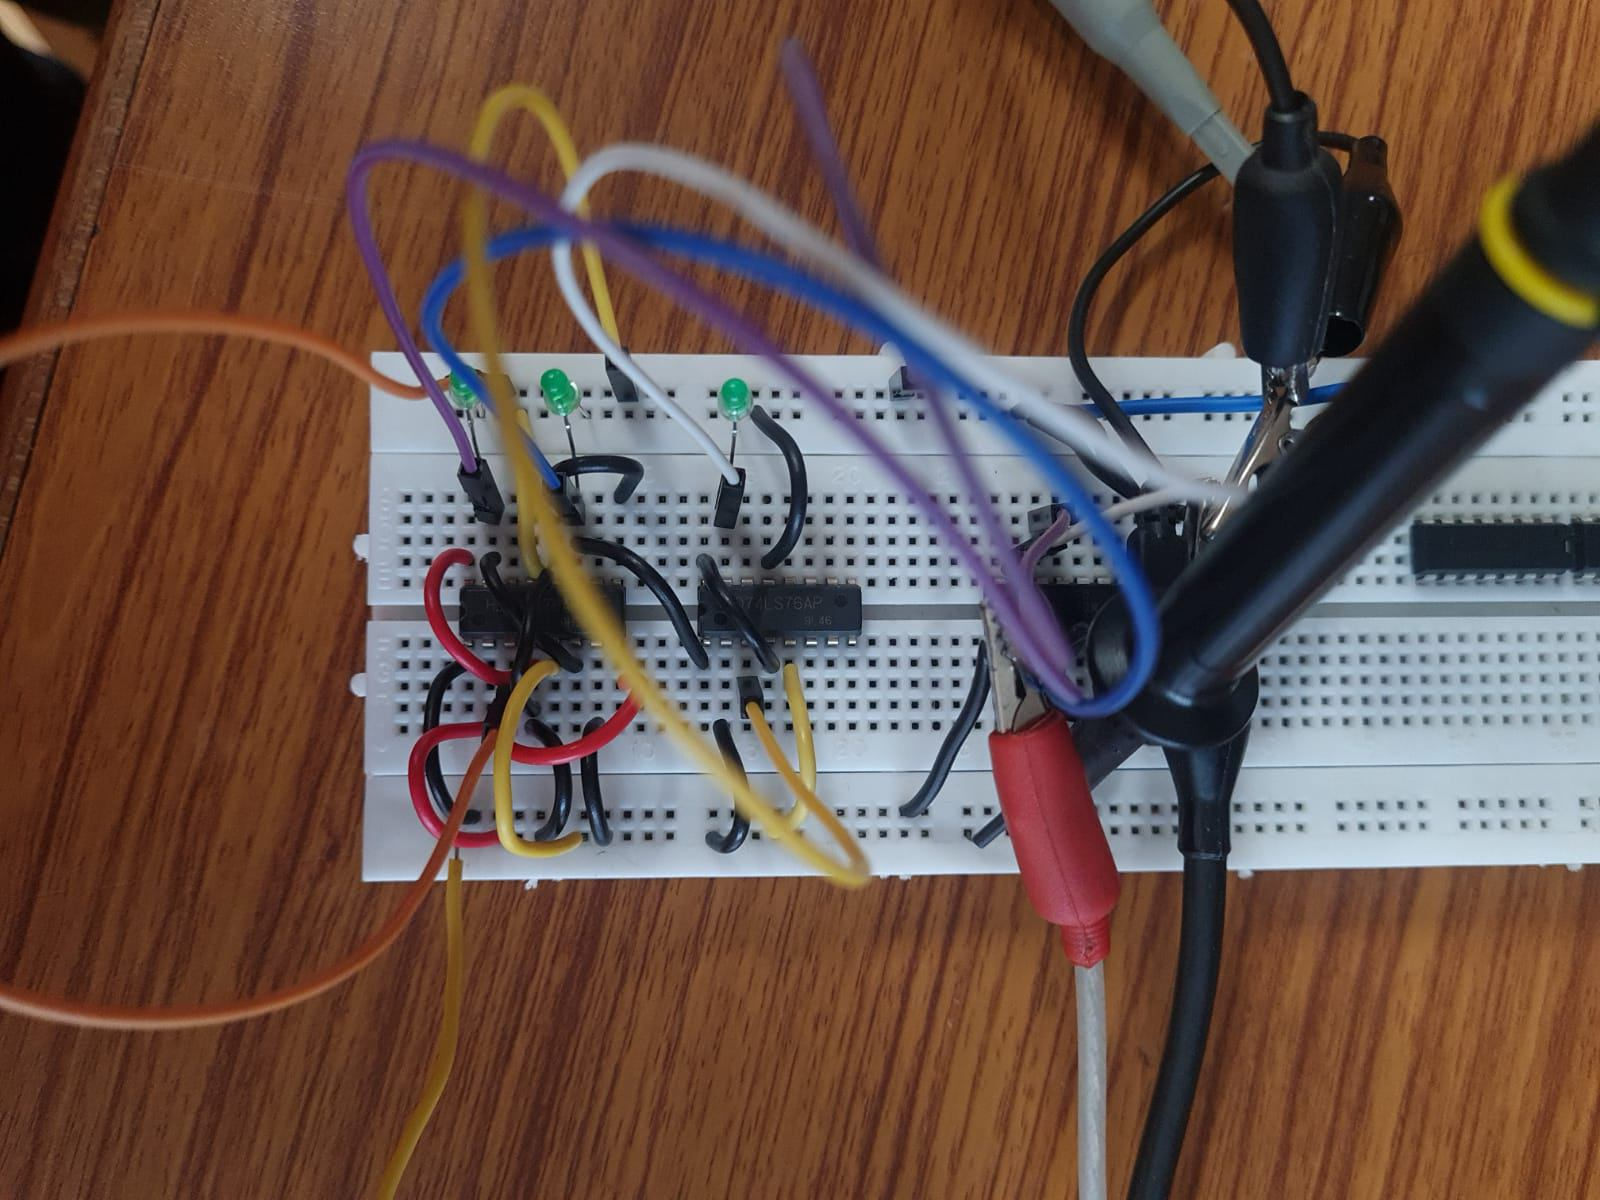
\includegraphics[width = 0.6\columnwidth]{figs/full.jpeg}
    \caption{The Circuit}
\end{figure}
\begin{figure}[H]
    \centering
    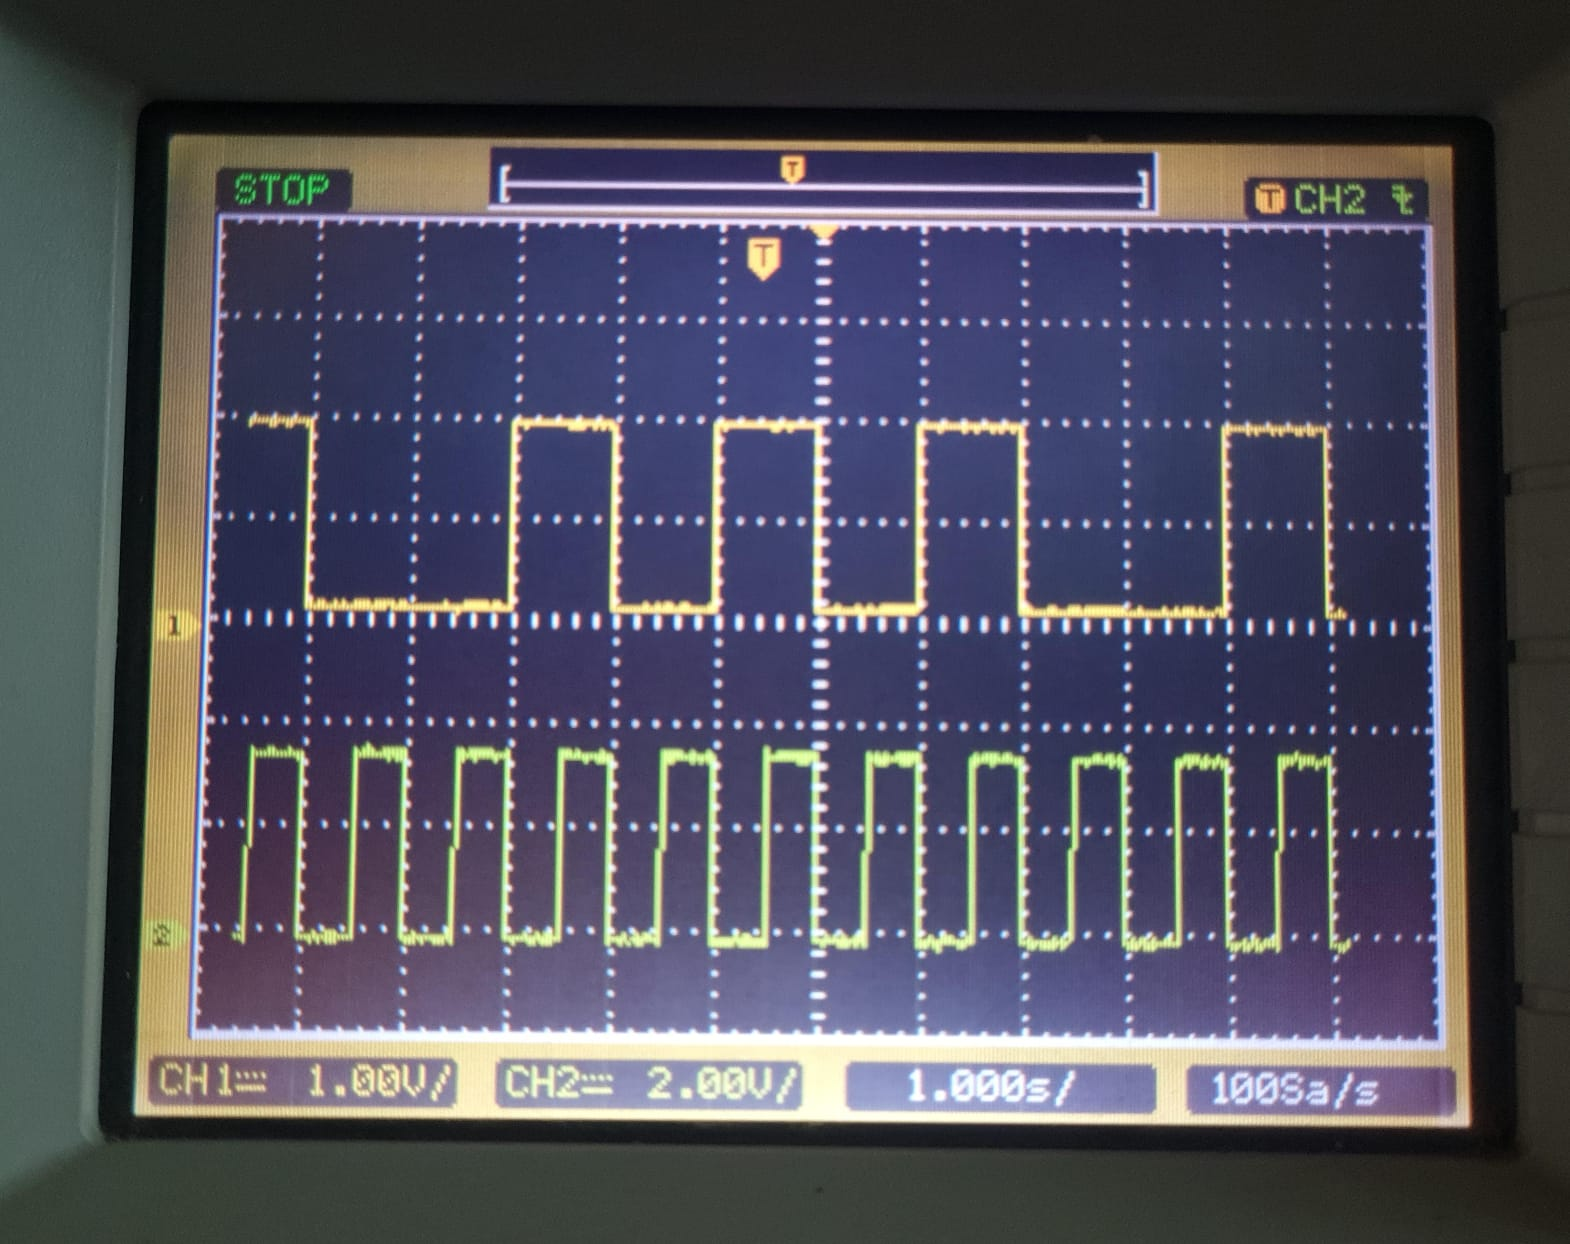
\includegraphics[width = 0.6\columnwidth]{figs/q1.jpeg}
    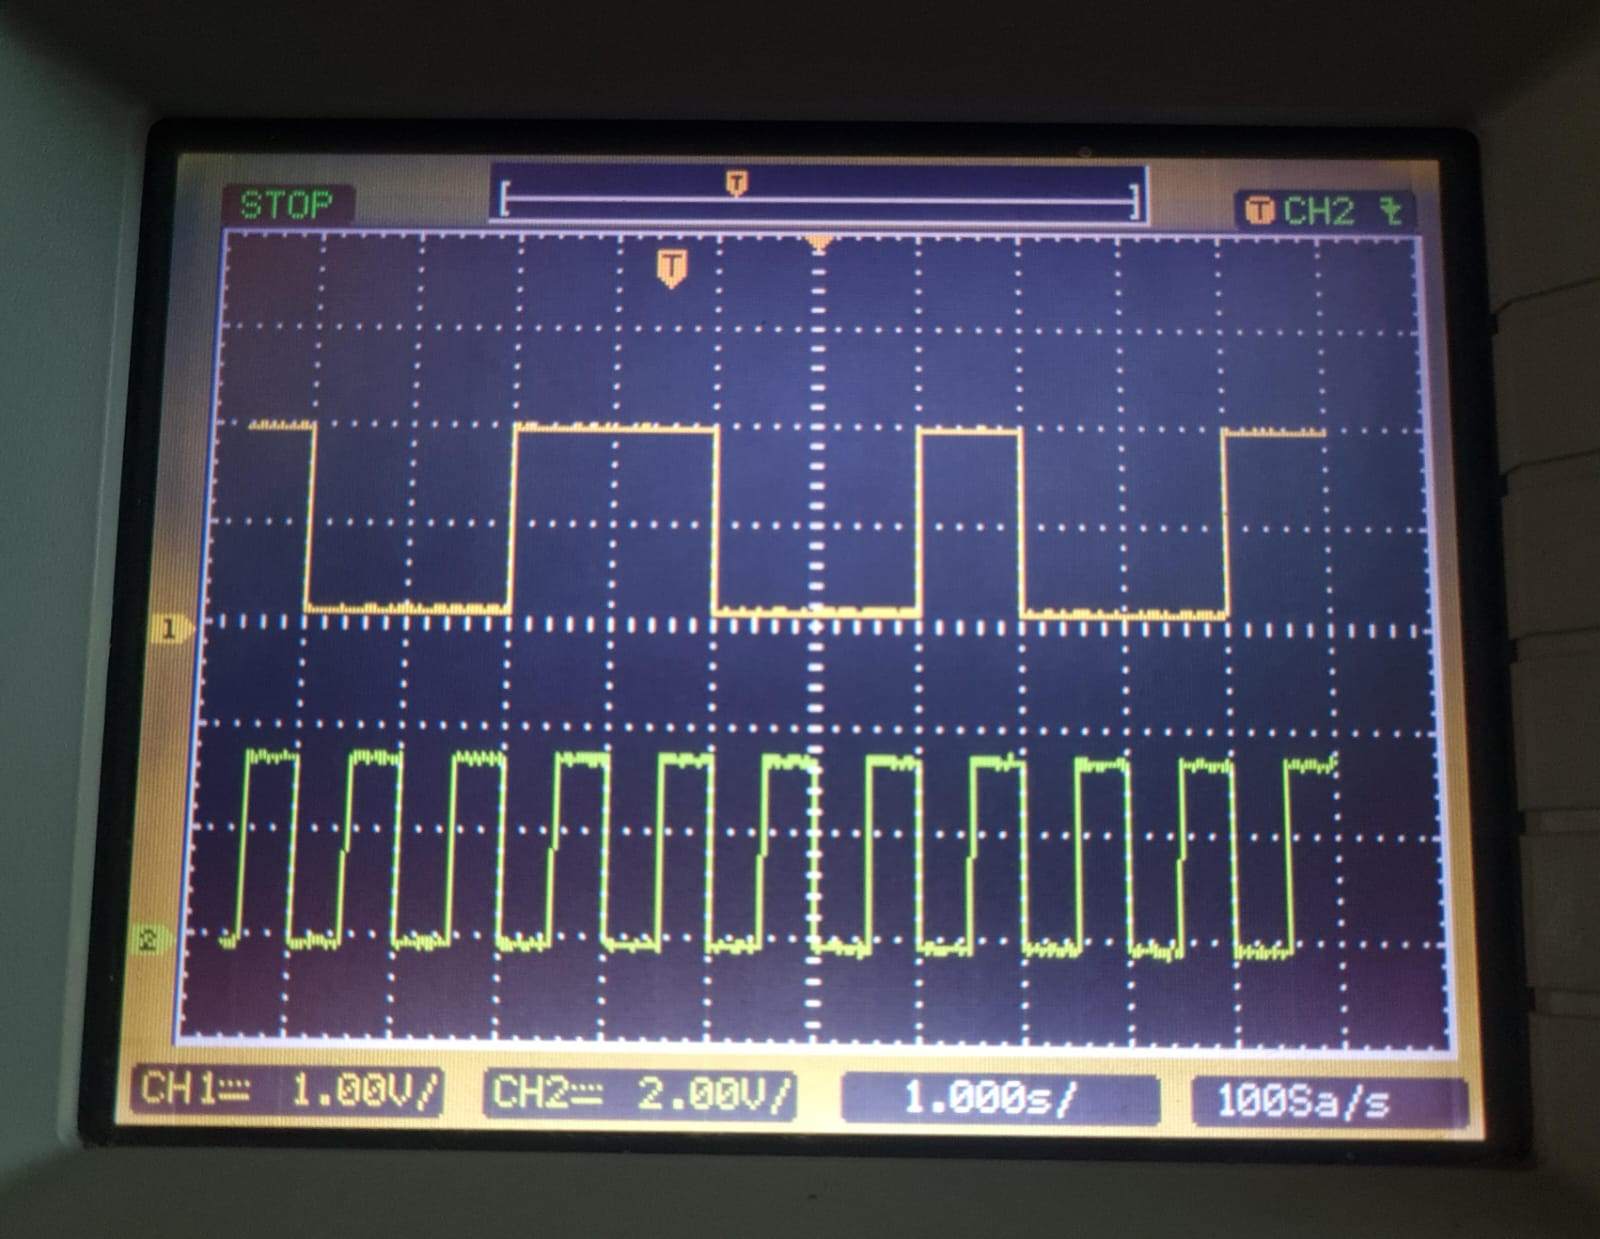
\includegraphics[width = 0.6\columnwidth]{figs/q2.jpeg}
    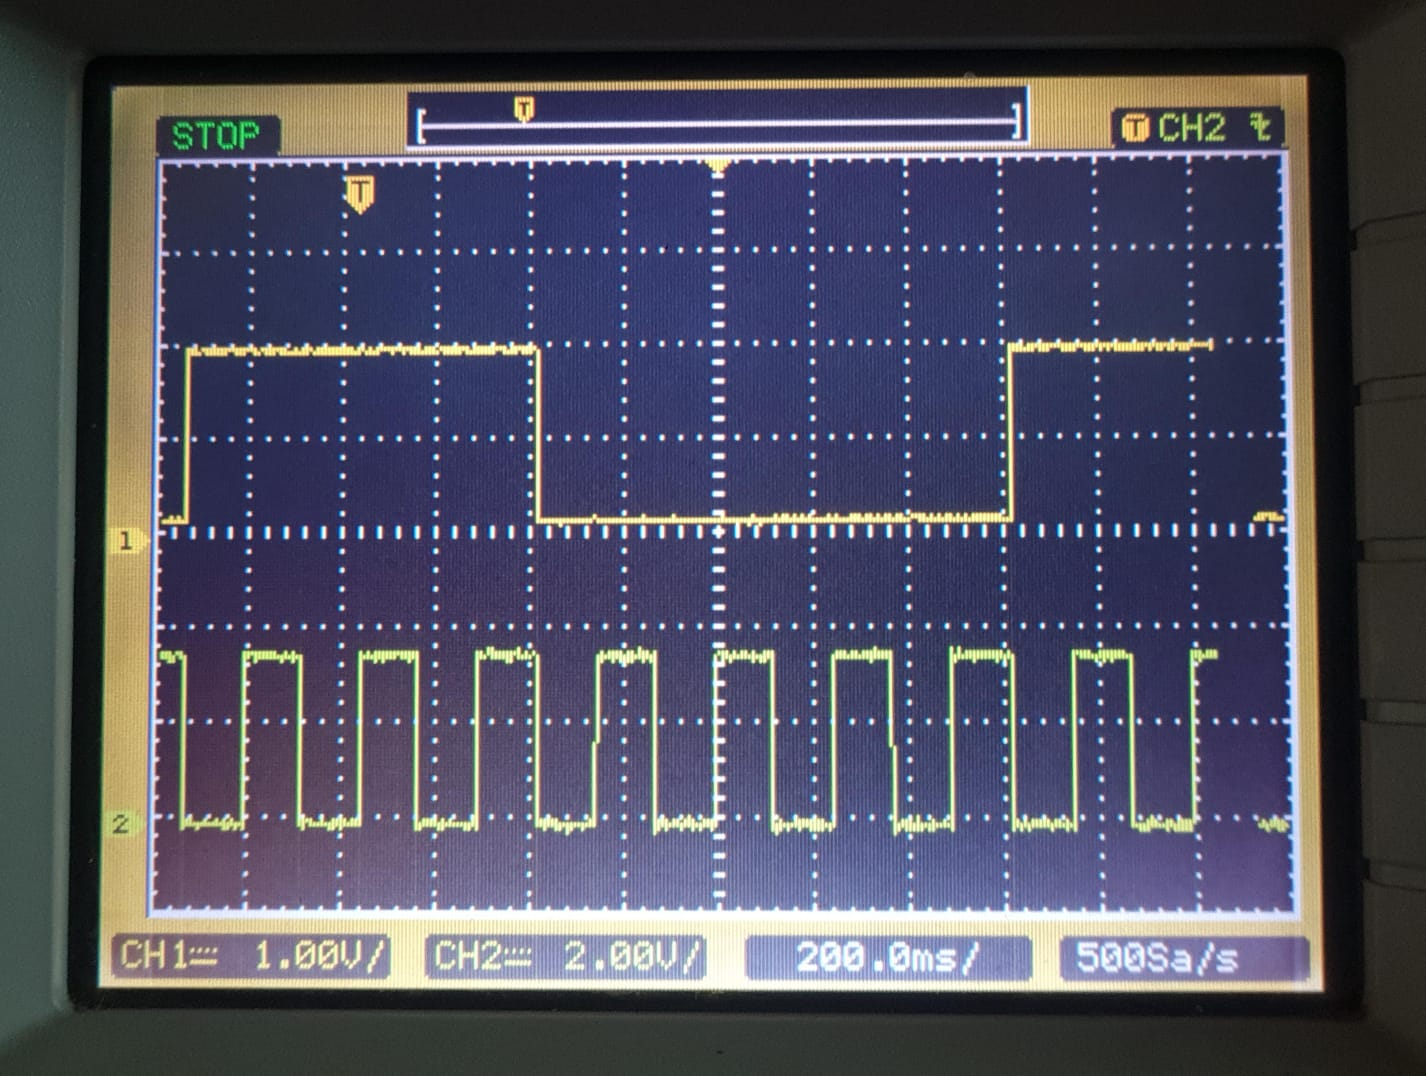
\includegraphics[width = 0.6\columnwidth]{figs/q3.jpeg}
    \caption{The signals $Q_0$, $Q_1$, $Q_2$ plotted with the initial clock signal, respectively.}
\end{figure}

As shown in the images above, we get the following state sequence in our circuit.

\begin{table}[H]
\centering
\begin{tabular}{cccccc}
\toprule
\textbf{Count} & \textbf{Q2} & \textbf{Q1} & \textbf{Q0} & \textbf{Decimal Equivalent} & \textbf{LED State} \\
\midrule
0 & 0 & 0 & 0 & 0 & Off-Off-Off \\
1 & 0 & 0 & 1 & 1 & Off-Off-On \\
2 & 0 & 1 & 0 & 2 & Off-On-Off \\
3 & 0 & 1 & 1 & 3 & Off-On-On \\
4 & 1 & 0 & 0 & 4 & On-Off-Off \\
5 & 1 & 0 & 1 & 5 & On-Off-On \\
6 & 1 & 1 & 0 & 6 & On-On-Off \\
7 & 0 & 0 & 0 & 0 (Reset) & Off-Off-Off \\
\bottomrule
\end{tabular}
\caption{State Sequence of our Mod-7 Counter, as shown on the LEDs}
\label{tab:states}
\end{table}

\section{Conclusion}
The sequential circuit functioned like a mod-7 counter, with the Arduino providing clock signal. 
\end{document}
